\section{Wednesday, October 2, 2019}

Last time, we finished generic programming. Today we'll talk about Java's Collections framework and then we'll start Linked Lists.

\subsection{Collections}

A \vocab{collection} is a group of individual objects represented as a single unit. For instance, sets, lists, queues, and ArrayLists are all collections since they allow us to store several elements (individual objects) inside of them. 

A \vocab{data structure} is a class that is used to represent and store information in a specific manner. Different data structures allow us to solve problems in different ways. The choice of data structure is important since it affects the abstractions supported, amount of storage required, and which operations can be performed efficiently. Collections can be implemented using many different data structures. For instance, a stack can be implemented using a array, \verb!ArrayList!, \verb!LinkedList!, and more. It's important to use the data structures provided in Java's Collections framework whenever possible (coding something up yourself from scratch may introduce errors).

The following image depicts the collections framework's hierarchy (these are ``is-a" relationships):

\begin{figure}[h]
\caption{Example of a parametric plot ($\sin (x), \cos(x), x$)}
\centering
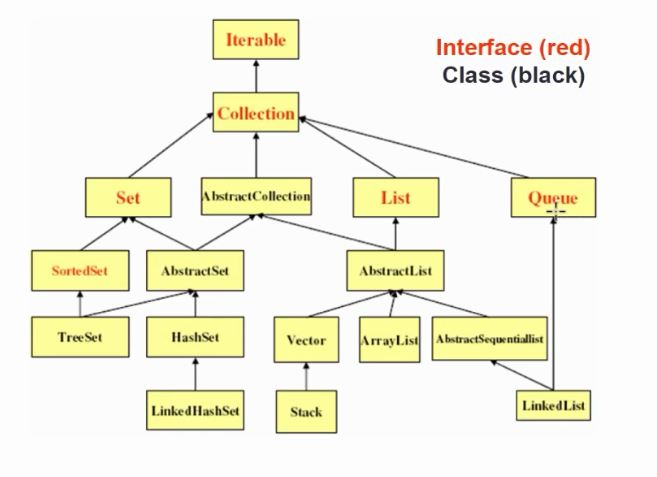
\includegraphics[width=0.75\textwidth]{media/hierarchy.jpg}
\end{figure}

Some interesting things to note are listed below:
\begin{itemize}
    \item Stacks are implemented internally using \verb!List! objects. This means that it is perfectly valid to pass in a stack into a function that expects a \verb!List!. 
    \item The \verb!LinkedList! class implements the \verb!Queue! interface. 
    \item Everything in the collections framework implements the \verb!Collection! interface. This means that a declaration like \verb!Collection<String> l = new ArrayList<String>()! is perfectly valid.
    \item Everything in the collections framework implements the \verb!Iterable! interface. This means that a declaration like \verb!Iterable<String> l = new ArrayList<String>()! is perfectly valid.
\end{itemize}



\subsection{Introduction to Linked Lists}  
A \vocab{Linked List} is a linear data structure that is composed of several \vocab{nodes}, each of which contain some data and a reference to the next node in the list. For example, the following figure illustrates a Linked List consisting of three integers: $12$, $99$, and $37$. 

\begin{figure}[h]
\centering
\begin{tikzpicture}[list/.style={rectangle split, rectangle split parts=2,
    draw, rectangle split horizontal}, >=stealth, start chain]

  \node[list,on chain] (A) {12};
  \node[list,on chain] (B) {99};
  \node[list,on chain] (C) {37};
  \node[on chain,draw,inner sep=6pt] (D) {};
  \draw (D.north east) -- (D.south west);
  \draw (D.north west) -- (D.south east);
  \draw[*->] let \p1 = (A.two), \p2 = (A.center) in (\x1,\y2) -- (B);
  \draw[*->] let \p1 = (B.two), \p2 = (B.center) in (\x1,\y2) -- (C);
  \draw[*->] let \p1 = (C.two), \p2 = (C.center) in (\x1,\y2) -- (D);
\end{tikzpicture}
\caption{A Linked List}
\end{figure}

The entire figure above represents a Linked List, and each individual square represents a square. Visually, we represent the end of a Linked List by a null reference (above, this is represented with a crossed out square).  

As shown in the above figure, it's important to remember that each node consists of two entities: the data stored in that node as well as a reference to the next node. 

In Java, we can implement a Linked List using an inner class to represent the node. Part of an implementation is shown below:

\begin{lstlisting}
package myLinkedList;

public class MyLinkedList<T extends Comparable<T>> { /* Notice the parameter */
	private class Node {
		private T data;
		private Node next;

		private Node(T data) {
			this.data = data;
			next = null; /* do we really need to do this? */
		}
	}

	/* List head pointer */
	private Node head;

	/* We don't actually need it */
	public MyLinkedList() {
		head = null;
	}

	/* Adding at the front of the list */
	public MyLinkedList<T> add(T data) {
		Node newNode = new Node(data);
		newNode.next = head;
		head = newNode;

		return this;
	}
\end{lstlisting}

As described earlier, each \verb!Node! object has a generic \verb!data! field to store some information as well as \verb!next! field, which stores the next \verb!Node! object in the Linked List. This may seem confusing at first since the definition of a \verb!Node! object includes a \verb!Node! field inside of it. This self-reference is permitted by Java. 